\xiti
\begin{xiaotis}

\xiaoti{什么叫平行直线?什么叫异面直线?说出它们的共同点和区别。}

\xiaoti{直线 $a$ 和两条异面直线 $b$、$c$ 都相交,画出每两条相交直线所确定的平面,并标上字母。}

\xiaoti{有三条直线,每两条都成异面直线。画出这三条直线。}

\xiaoti{在一块长方体形木块的 $A_1C_1$ 面上有一点 $P$,
    过点 $P$ 画一条直线和棱 $CD$ 平等,说明应该怎样画。
}

\begin{figure}[htbp]
    \centering
    \begin{minipage}[b]{5cm}
        \centering
        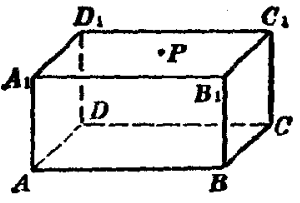
\includegraphics[width=5cm]{../pic/ltjh-ch1-xiti2-04.png}
        \caption*{(第 4 题)}
    \end{minipage}
    \qquad
    \begin{minipage}[b]{4cm}
        \centering
        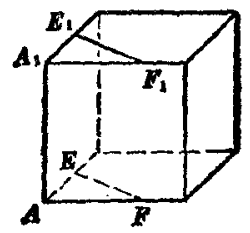
\includegraphics[width=4cm]{../pic/ltjh-ch1-xiti2-05.png}
        \caption*{(第 5 题)}
    \end{minipage}
    \qquad
    \begin{minipage}[b]{5cm}
        \centering
        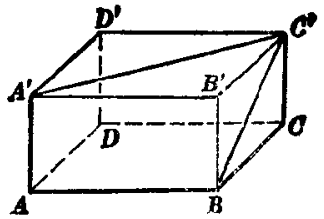
\includegraphics[width=5cm]{../pic/ltjh-ch1-xiti2-11.png}
        \caption*{(第 11 题)}
    \end{minipage}
\end{figure}

\xiaoti{如图,在正方体中, $AE =A_1E_1$, $AF = A_1F_1$。
    求证:$EF \pxqdy E_1F_1$。
}

\xiaoti{已知: $E$、$F$、$G$、$H$ 分别是空间四边形的四条边 $AB$、$BC$、$CD$、$DA$ 的中点。
    求证:四边形 $EFGH$ 是平行四边形。
}

\xiaoti{已知:直线 $a$ 和 $b$ 是异面直线,直线 $c \pingxing a$, 直线 $b$ 与 $c$ 不相交。
    求证: 直线 $b$、$c$ 是异面直线。
}

\xiaoti{分别和两条异面直线 $AB$、$CD$ 同时相交的两条直线 $AC$、$BD$ 一定是异面直线。为什么?}

\xiaoti{什么叫两条异面直线所成的角?两条异面直线在什么情况下互相垂直?}

\xiaoti{}%
\begin{xiaoxiaotis}%
    \xxt[\xxtsep]{求证:如果一条直线和两条平行线中的一条垂直,那么也和另一条垂直。}

    \xxt{某一条直线与两条平行直线都不相交,且与其中一条所成的角等于 $\theta$,
        则该直线与另一条直线所成的角也等于 $\theta$。
    }

\end{xiaoxiaotis}

\xiaoti{如图,已知长方体的长和宽都是 4 cm,高是 2 cm。
    (1) $BC$ 和 $A'C'$ 所成的角是多少度?
    (2) $AA'$ 和 $BC'$ 所成的角是多少度?
    (3) $A'B'$ 和 $DD'$; $B'C'$ 和 $CD$ 的距离各是多少?
}

\end{xiaotis}

